\section{Szereg Fouriera}
\subsection{Definicja}
Niech funkcja \textbf{f} będzie określona na odcinku $\mathbf{\left[-\frac{T}{2}, \frac{T}{2}\right]}$ poza skończoną liczbą punktów oraz będzie określona poza przedziałem $\mathbf{\left[-\frac{T}{2}, \frac{T}{2}\right]}${\tiny } poprzez równość $\mathbf{f(x) = f(x + T)}$ (okresowość)
\\ \\
\textbf{Trygonometrycznym szeregiem Fouriera} funkcji f nazywamy szereg funkcyjny następującej postaci:
$$S(x) = \frac{a_{0}}{2} + \sum_{n=1}^{\infty} \left(a_{n} cos\left(\frac{2n\pi}{T} x\right) + b_{n} sin\left(\frac{2n\pi}{T} x\right) \right)$$
O współczynnikach określonych następującymi wzorami:
$$ a_{n} = \frac{2}{T} \int_{-\frac{T}{2}}^{\frac{T}{2}} f(x)cos\left(\frac{2n\pi}{T} x \right) dx,	\quad n = 0,1,2,...$$

$$ b_{n} = \frac{2}{T} \int_{-\frac{T}{2}}^{\frac{T}{2}} f(x)sin\left(\frac{2n\pi}{T} x \right) dx,	\quad n = 1,2,3,...$$


\subsection{Cel ćwiczenia}
Zadane funkcje na określonych przedziałach rozwinęliśmy w szereg Fouriera oraz narysowaliśmy ich wykresy dla \textbf{n = 100}.

\begin{itemize}
    \item $f(x) = x, \quad x\in [-1,1]$
    
    \item $f(x) = x^{2}, \quad x\in [0,1]$
    
    \item $f(x) = sin(x), \quad x\in [-\pi,\pi]$
\end{itemize}

\subsection{Algorytm}
\vspace*{0.1cm}
Poniżej został zaprezentowany kod programu w języku Python:\\

\begin{Shaded}
\begin{Highlighting}[]
\ImportTok{import} \NormalTok{numpy }\ImportTok{as} \NormalTok{np}
\ImportTok{import} \NormalTok{matplotlib.pyplot }\ImportTok{as} \NormalTok{plt}
\KeywordTok{def} \NormalTok{series(x):}
    \NormalTok{const }\OperatorTok{=} \DecValTok{2} \OperatorTok{*} \NormalTok{np.pi }\OperatorTok{*} \NormalTok{x }\OperatorTok{/} \NormalTok{T}
    \ControlFlowTok{return} \KeywordTok{lambda} \NormalTok{x: An(n) }\OperatorTok{*} \NormalTok{np.cos(const }\OperatorTok{*} \NormalTok{n) }\OperatorTok{+} \NormalTok{Bn(n) }\OperatorTok{*} \NormalTok{np.sin(const }\OperatorTok{*} \NormalTok{n)}
\KeywordTok{def} \NormalTok{fab1():}
    \ControlFlowTok{return} \KeywordTok{lambda} \NormalTok{n: }\DecValTok{0}\NormalTok{, }\KeywordTok{lambda} \NormalTok{n: (}\OperatorTok{-}\DecValTok{2}\OperatorTok{*}\NormalTok{(}\OperatorTok{-}\DecValTok{1}\NormalTok{)}\OperatorTok{**}\NormalTok{n)}\OperatorTok{/}\NormalTok{(np.pi }\OperatorTok{*} \NormalTok{n)}
\KeywordTok{def} \NormalTok{fab2():}
    \ControlFlowTok{return} \KeywordTok{lambda} \NormalTok{n: }\DecValTok{1}\OperatorTok{/}\NormalTok{(np.pi}\OperatorTok{**}\DecValTok{2} \OperatorTok{*} \NormalTok{n}\OperatorTok{**}\DecValTok{2}\NormalTok{), }\KeywordTok{lambda} \NormalTok{n: }\OperatorTok{-}\DecValTok{1}\OperatorTok{/}\NormalTok{(np.pi }\OperatorTok{*} \NormalTok{n)}
\KeywordTok{def} \NormalTok{fab3():                                                              }
    \ControlFlowTok{return} \KeywordTok{lambda} \NormalTok{n: }\DecValTok{0}\NormalTok{, }\KeywordTok{lambda} \NormalTok{n: }\DecValTok{1} \ControlFlowTok{if} \NormalTok{n}\OperatorTok{==}\DecValTok{1} \ControlFlowTok{else} \DecValTok{0}   
\KeywordTok{def} \NormalTok{fun():}
    \ControlFlowTok{return} \KeywordTok{lambda} \NormalTok{x: x, }\KeywordTok{lambda} \NormalTok{x: x}\OperatorTok{**}\DecValTok{2}\NormalTok{, }\KeywordTok{lambda} \NormalTok{x: np.sin(x)}
\KeywordTok{def} \NormalTok{plotSeries(x, S, fx):}
    \NormalTok{fig }\OperatorTok{=} \NormalTok{plt.figure()}
    \NormalTok{ax }\OperatorTok{=} \NormalTok{fig.add_subplot(}\DecValTok{111}\NormalTok{)}
    \NormalTok{ax.plot(x, S, x, fx(x), }\StringTok{'r--'}\NormalTok{)}
    \NormalTok{plt.show()}
\NormalTok{rng = int(input('Wpisz range: '))}
\NormalTok{A }\OperatorTok{=} \NormalTok{[}\OperatorTok{-}\DecValTok{1}\NormalTok{, }\DecValTok{0}\NormalTok{, }\OperatorTok{-}\NormalTok{np.pi]}
\NormalTok{B }\OperatorTok{=} \NormalTok{[}\DecValTok{1}\NormalTok{, }\DecValTok{1}\NormalTok{, np.pi]}
\NormalTok{A0 }\OperatorTok{=} \NormalTok{[}\DecValTok{0}\NormalTok{, }\DecValTok{2}\OperatorTok{/}\DecValTok{3}\NormalTok{, }\DecValTok{0}\NormalTok{] }
\NormalTok{F }\OperatorTok{=} \NormalTok{\{}\StringTok{"x"} \NormalTok{: [fab1()], }\StringTok{"x^2"} \NormalTok{: [fab2()], }\StringTok{"sin(x)"} \NormalTok{: [fab3()]\}}
\NormalTok{fx }\OperatorTok{=} \NormalTok{[fun()]}
\NormalTok{X }\OperatorTok{=} \NormalTok{[]}
\NormalTok{Tt }\OperatorTok{=} \NormalTok{[]}
\ControlFlowTok{for} \NormalTok{i }\OperatorTok{in} \BuiltInTok{range}\NormalTok{(}\DecValTok{3}\NormalTok{):}
    \NormalTok{X.append(np.linspace(A[i], B[i], num}\OperatorTok{=}\DecValTok{1000}\NormalTok{))}
    \NormalTok{Tt.append(B[i] }\OperatorTok{-} \NormalTok{A[i])}
\NormalTok{X }\OperatorTok{=} \NormalTok{np.array(X)}
\NormalTok{Tt }\OperatorTok{=} \NormalTok{np.array(Tt)}
\ControlFlowTok{for} \NormalTok{inx, (k, v) }\OperatorTok{in} \BuiltInTok{enumerate}\NormalTok{(F.items()):}
    \NormalTok{a }\OperatorTok{=} \NormalTok{A[inx] }
    \NormalTok{b }\OperatorTok{=} \NormalTok{B[inx]}
    \NormalTok{a0 }\OperatorTok{=} \NormalTok{A0[inx]}
    \NormalTok{T }\OperatorTok{=} \NormalTok{Tt[inx] }
    \NormalTok{x }\OperatorTok{=} \NormalTok{X[inx]}
    \NormalTok{An, Bn }\OperatorTok{=} \NormalTok{v[}\DecValTok{0}\NormalTok{][}\DecValTok{0}\NormalTok{], v[}\DecValTok{0}\NormalTok{][}\DecValTok{1}\NormalTok{]}
    \NormalTok{f }\OperatorTok{=} \NormalTok{series(x)}
    \NormalTok{S }\OperatorTok{=} \NormalTok{np.zeros((x.shape))}
    \ControlFlowTok{for} \NormalTok{i }\OperatorTok{in} \BuiltInTok{range}\NormalTok{(}\DecValTok{1}\NormalTok{, rng}\DecValTok{+1}\NormalTok{):}
        \NormalTok{n }\OperatorTok{=} \NormalTok{i}
        \NormalTok{S }\OperatorTok{+=} \NormalTok{f(x)}
    \NormalTok{S }\OperatorTok{+=} \NormalTok{a0}\OperatorTok{/}\DecValTok{2}
    \NormalTok{plotSeries(x,S, fx[}\DecValTok{0}\NormalTok{][inx])}
\end{Highlighting}
\end{Shaded}
\subsection{Wykresy}
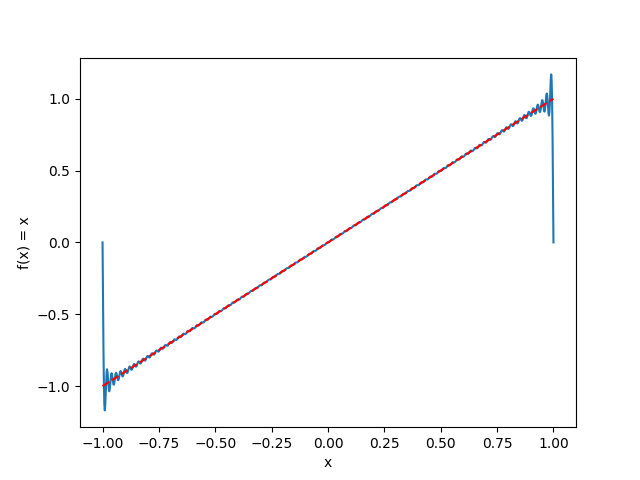
\includegraphics{Lab1/charts/Figure_1.png}

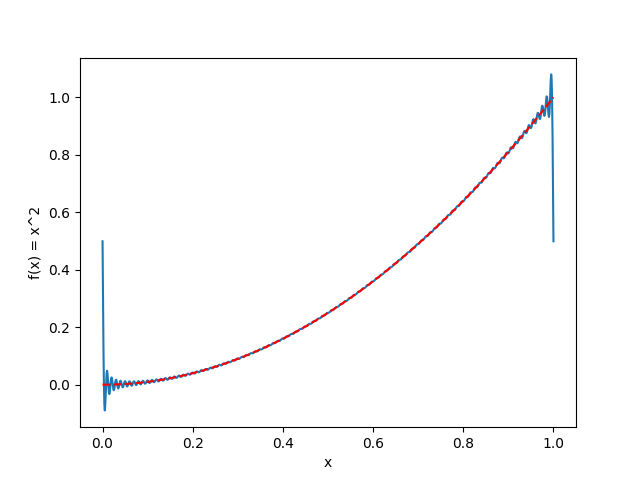
\includegraphics{Lab1/charts/Figure_2.png}
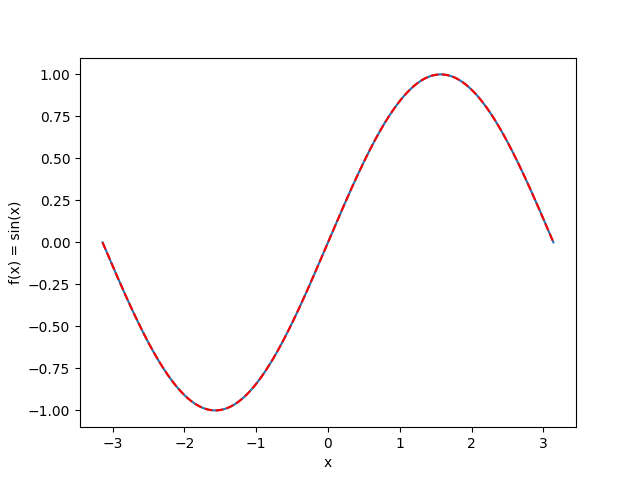
\includegraphics{Lab1/charts/Figure_3.png}
